\documentclass[a4paper]{exam}

\usepackage{graphicx}
\usepackage{hyperref}
\usepackage{tabularx}
\usepackage{tikz}

\printanswers

\title{Weekly Challenge 07: Playing Registrar}
\author{CS/CE 412/471 Algorithms: Design and Analysis}
\date{Spring 2025}

\begin{document}
\maketitle
\thispagestyle{empty}

\section*{Purpose}

In this WC, you will model exam scheduling as a \textit{graph coloring} problem using a \textit{conflict graph}, transforming exam scheduling into a \textit{combinatorial optimization} problem. This reinforces key algorithmic concepts such as graph representation, graph coloring, and combinatorial optimization. The problem closely mirrors real-world scheduling challenges in university timetabling, operating systems, and resource allocation.

\subsection*{Skills}

This WC builds your skills in problem-solving and quantitative reasoning, invites you to apply computational thinking to real-world problems, and reinforces your skills related to algorithmic problem-solving and analysis. These align with the university's  \href{https://habib.edu.pk/about-us/vision-values/}{learning goals}, the CS program's \href{https://habib.edu.pk/academics/sse/computer-science/}{learning outcomes}, and the course's \href{https://hulms.instructure.com/courses/4297/outcomes}{learning objectives}.

Problems similar to the one described in this WC arise in real-world scheduling problems (e.g., timetabling, task scheduling, and resource allocation) and are widely applicable in job scheduling in operating systems, network optimization, and artificial intelligence.

Applying computer science concepts and computational thinking to real world problems in this manner will make you a more capable and versatile computer scientist.

Specifically, this WC develops expertise in:
\begin{itemize}
\item Graph Representation and Modeling: building a conflict graph from student enrollment data
\item Graph Coloring Algorithms: using graph coloring to minimize exam slots
\item Algorithm Design and Justification: developing and implementing an efficient scheduling algorithm
\item Data Visualization: using Python libraries to visualize conflict graphs
\item Computational Thinking and Randomization: generating realistic random course enrollment data
\end{itemize}

\section*{Background and Requirements}

To attempt and submit the WC, you will require:
\begin{itemize}
\item An understanding of graphs
\item The ability to apply algorithmic thinking to solve a problem
\item The ability to program in Python and to read and follow technical tutorials
\item Working knowledge of \LaTeX
\end{itemize}

\begin{center}
  \rule{300pt}{1pt}
  
    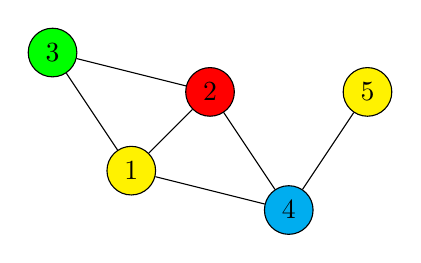
\begin{tikzpicture}[baseline=(current bounding box.north)]
\node[draw, circle, fill=yellow] at (0,0) (1) {1};
\node[draw, circle, fill=red] at (1,1) (2) {2};
\node[draw, circle, fill=green] at (-1,1.5) (3) {3};
\node[draw, circle, fill=cyan] at (2,-0.5) (4) {4};
\node[draw, circle, fill=yellow] at (3,1) (5) {5};

\draw (1) to (2) to (3) to (1) to (4) to (2);
\draw (4) to (5);
\end{tikzpicture}
\end{center}
\newpage
\section*{The Setup}

A \textit{graph} $G= (V, E)$ consists of $V$, a nonempty set of \textit{vertices} (or \textit{nodes}), and $E$, a set of \textit{edges} (or \textit{links}). Each edge is a set of unordered pairs $\{v_1, v_2\}$ of vertices. The vertices $v_i$ and $v_2$ of an edge $\{v_i, v_2\}$ are called the edge's \textit{endpoints}. 

Of course, as a capable student of Algorithms, you already know this! Moreover, Registrar Office (RO) knows that you know this, and is seeking your help to schedule final exams.

You are provided the data of $n$ courses, each of which requires an exam to be scheduled. For each course, $i$, $1\le i \le n$, you are also provided the data of all the students enrolled in the course. Specifically, you are provided the student IDs of the enrolled students.

RO wants you to schedule exams such that every student can take their exam. That is, every student takes the final exam of every course that they are enrolled in and no student has more than one exam scheduled at any given time. RO also wants you to minimize the total number of time slots in which exams are scheduled.

Employing your algorithmic prowess, you come up with a \textit{conflict graph}. It is a graph containing $n$ nodes, where each node represents an exam to be scheduled. Two nodes have an edge between them iff the corresponding courses \textit{conflict}, i.e., they cannot be scheduled at the same time because there is at least one student who is enrolled in both of them.

Remembering the saying, ``the world isn't just black and white'', from your Core courses, you have decided to assign colors to time slots in your conflict graph. All courses whose nodes have the same color in the graph will be scheduled at the same time.

Thus, you have transformed your scheduling task to a \textit{graph coloring} problem! You just have to figure out the minimum number of colors to assign to your nodes such that the endpoints of any given edge have a different color. Feeling smart, happy, and humbled, you make a pilgrimage to \href{https://en.wikipedia.org/wiki/Al-Khwarizmi_Complex}{Uzbekistan} in order to honor \href{https://www.openculture.com/2022/04/why-algorithms-are-called-algorithms.html}{Al-Khwarizmi}.


\section*{Example}

Shown below on the left is sample enrollment data of 5 courses, where the $i$-th line contains the student IDs of the students enrolled in course $i$. On its right is a resulting conflict graph of the exams. The graph is colored. The graph shows that course 1 conflicts with courses 2, 3, and 4; course 2 conflicts with courses 1, 3, and 4; and so on. A total of 4 time slots (colors) are used. Exams for course 1 and course 5 take place in the same time slot. All of the other exams take place in different, separate time slots.
\bigskip

\begin{minipage}{.4\textwidth}
\begin{itemize}
\item S1, S3, S6, S13, S17, S18
\item S4, S7, S9, S14, S17, S18
\item S1, S2, S6, S7, S12
\item S3, S4, S5, S8, S9, S16
\item S5, S8, S19, S20
\end{itemize}
\end{minipage}
\begin{minipage}{.4\textwidth}
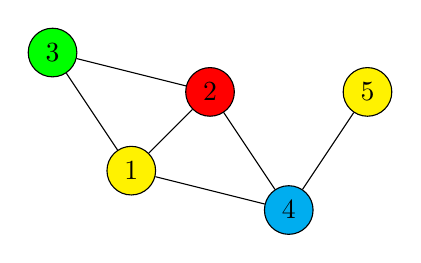
\begin{tikzpicture}[baseline=(current bounding box.north)]
\node[draw, circle, fill=yellow] at (0,0) (1) {1};
\node[draw, circle, fill=red] at (1,1) (2) {2};
\node[draw, circle, fill=green] at (-1,1.5) (3) {3};
\node[draw, circle, fill=cyan] at (2,-0.5) (4) {4};
\node[draw, circle, fill=yellow] at (3,1) (5) {5};

\draw (1) to (2) to (3) to (1) to (4) to (2);
\draw (4) to (5);
\end{tikzpicture}
\end{minipage}
\section*{Tasks}

\begin{questions}

\question
  Given a conflict graph with $n$ nodes, what is the \textit{maximum} number of colors that you can use to color your nodes such that neighboring nodes have different colors? Justify your answer.
  \begin{solution}
    
  \end{solution}
\question
  Of course, RO is interested in the \textit{minimum} number of colors. What is the minimum number of colors that can be used in a conflict graph with $n$ nodes? Justify your answer.
  \begin{solution}
    
  \end{solution}

\question
  Devise an algorithm to assign the minimum number of colors to the nodes in a conflict graph. Provide the algorithm here in CLRS format.
  \begin{solution}
    
  \end{solution}

\question
  Provide below, sample enrollment data for a desired number, $n$, of courses. The $i$-th line, $1\le i\le n$, contains the student IDs of the students enrolled in course $i$. Ensure a good amount of cross-enrollment, i.e., students enrolled in multiple and overlapping courses.
  \begin{solution}
    
  \end{solution}

\question
  Include below a visualization of your conflict graph which is colored according to your algorithm above. Make sure that each node is labeled with its course ID.
  \begin{solution}
    
  \end{solution}

  \bonusquestion (Optional, no points)
  Include below a picture or drawing of you honoring Al-Khwarizmi. The picture may be hand drawn. Al-Khwarizmi would probably feel more honored if it were algorithmically generated.
  \begin{solution}
    
  \end{solution}  
\end{questions}

\section*{Hints}
\begin{itemize}
\item Use the \texttt{networkx} package in Python to model a graph and the \texttt{matplotlib} package to visualize it. You can find related instructions \href{https://www.geeksforgeeks.org/python-visualize-graphs-generated-in-networkx-using-matplotlib/}{here}.
\item Instructions on adding color to the visualization are available \href{https://stackoverflow.com/questions/27030473/how-to-set-colors-for-nodes-in-networkx}{here}.
\end{itemize}

\section*{Submission}

Fill in the solution boxes above and submit the generated PDF file.


\end{document}

%%% Local Variables:
%%% mode: latex
%%% TeX-master: t
%%% End:
